% CHILL ZEN, condensed. A big-picture companion to main.tex for
% technical readers, executives, and investors. No new experiments:
% every number here is taken from main.tex and traces to NUMBERS.md.
% Build: tectonic main-short-fable.tex
\documentclass[reprint,amsmath,amssymb,aps,nofootinbib]{revtex4-2}

\usepackage{graphicx}
\usepackage{booktabs}
\usepackage{array}
\usepackage[colorlinks,linkcolor=blue,citecolor=blue,urlcolor=blue]{hyperref}

\newcommand{\kB}{k_{B}}

\begin{document}

\title{CHILL ZEN in brief: generative AI from noisy memory reads}

\author{M. Alexander Nugent}
\affiliation{Knowm Inc.}

\date{\today}

\begin{abstract}
This is a condensed account of a longer technical paper on CHILL ZEN
(Comparator-Heated In-memory Lane Learning with Zero-Ended Noise), an
architecture that generates images inside memristor memory instead of
on a processor. Each image is produced by about 3600 noisy reads of
stored weights, with no equilibrium sampling phase. The randomness
comes mostly from the read comparator, whose noise is set by each read
instruction, so the same memory reads ``hot'' to draw and ``cold'' to
decide. In emulation on binarized Fashion-MNIST the system scores FID
18.1, or 9.7 when trained on binary images, against 24.9 for the
published eight-step Denoising Thermodynamic Model (DTM). Under the
stated energy models it uses about one eighth of the DTM's energy per
image. All results are emulated; the lane-scale hardware has not been
built. We state what has been shown, what is modeled, and what remains
to be demonstrated.
\end{abstract}

\maketitle

\section{Why this matters}

Generative AI is expensive because it samples. A diffusion model or an
energy-based model produces each output through a long chain of
randomized updates, and every update runs on a digital processor that
must manufacture its own randomness from deterministic logic. The
energy cost of that sampling has become a first-order constraint on
deployment \cite{conte2019thermodynamic}.

One response is to let physics do the sampling. Probabilistic bits
built from stochastic nanomagnets and subthreshold transistors have
solved optimization and learning problems at very low energy
\cite{sutton2017intrinsic,borders2019integer,niazi2024training}.
The most complete proposal to date is the Denoising Thermodynamic
Model and its hardware, the Denoising Thermodynamic Computer
Architecture (DTCA) \cite{jelincic2025dtm}. It chains two to eight
energy-based models, each sampled by a bank of transistor random-number
generators, and it reports both image quality and an energy budget.
That paper also names the central difficulty. A single energy-based
model that fits real data well develops deep energy barriers between
its modes, and any local sampler then takes a long time to mix between
them. Chaining models keeps each step easy to mix, but the chain still
needs on the order of ten million random updates per image.

CHILL ZEN takes a different route to the same goal. Instead of
reversing a noising process through equilibrium sampling, it draws an
image's discrete code in one fixed sequence of noisy memory reads and
then reconciles the code in one cold sweep. There is no mixing phase.
The randomness that makes each draw different is supplied at the point
where the memory is read, by a comparator whose noise level is part of
the read instruction. The full paper reports that this design, in
emulation, beats the published DTM on quality and on modeled energy at
once. This document explains how, and how much of that claim rests on
measurement versus modeling.

\section{The idea in one page}

\subsection{The memory element is also the sampler}

The storage element is a pair of memristors read through a voltage
divider. The pair's balance is the stored weight $w \in [-1, 1]$, and
the pair's total conductance is its magnitude $m$. Magnitude acts like
accumulated evidence: the more a pair has been taught, the less a
fixed feedback pulse moves it, and the less noise its read carries.

A read returns the weight plus noise. The noise has three sources. Two
are in the devices, thermal and flicker, and both fall as magnitude
grows. The third is the read comparator's own input-referred noise,
which does not depend on the stored state at all. The thermal term
scales inversely with read voltage, so a low-voltage read is hot and a
full-voltage read is cold. The sign of one hot read is a probabilistic
bit whose bias is the stored weight. The same physical element stores
the parameter and draws the sample.

\subsection{Lanes pool pairs, and pooling quenches device noise}

A neural lane pools many pairs on one shared divider. By Kirchhoff's
laws a lane reports the magnitude-weighted average of the selected
weights. Selection is an address: an ordered tuple of symbols, one per
address space, and each space contributes in proportion to its share
of the pooled magnitude. Lanes are grouped into winner-take-all groups,
one lane per symbol, and taught by a local three-case rule: read every
lane, reinforce the correct one, oppose a wrong one that fired, and
mildly reinforce a correctly silent one. There are no gradients and no
host in the loop for the banks. Taught this way, a cold argmax readout
is a classifier at parity with logistic regression on the same
encoding.

Pooling has a consequence that determines the whole design. As
hundreds of pairs are pooled, their device noise averages down to a
floor set by the output node's capacitance, the familiar kT/C limit. At
the assumed 10\,mV hot read the lanes supply less than 40\% of the
noise a useful draw needs on the first read and less than 10\%
thereafter. The devices cannot heat themselves enough to sample. The
comparator has to supply the temperature.

\subsection{The comparator sets the temperature}

Every comparator has input-referred noise, and circuit settings control
it: lower the preamplifier bias, add an input noise source, or trigger
the latch earlier. CHILL ZEN treats that setting as a trim register
written by each read instruction, alongside read voltage and pulse
width. A hot read uses low bias and a cold read uses full bias. The
two regimes occur within a single image. At the operating point the
comparator supplies more than 90\% of the draw's variance on every
read after the first. This is what the name means: the lanes are
heated by the comparator, and the noise is ended, zeroed, for the
final decision.

\subsection{The code and the generation procedure}

Images are represented by an additive discrete code: a fixed set of
codebooks whose selected atoms sum to the image through a fixed linear
decoder. The code is fitted on the host with a dropout objective, so
that partial codes decode to reasonable images and the address spaces
carry information about one another. The deployed system uses a
904-bit code: a global backbone of 128 books over the whole canvas and
a residual patch code on a $7 \times 7$ grid of slots, plus the
clamped class label. Stripped of the hardware, the model class sits
beside masked-token generation over a discrete codebook
\cite{chang2022maskgit,vandenoord2017vqvae}, with local teaching in
place of a transformer.

Each level pairs a soft generator bank, which draws with hot reads,
and a hard repair bank, which corrects with one cold parallel sweep.
Generation runs in five steps. Clamp the label. Draw the 128 backbone
books one at a time with hot reads, then apply one cold repair sweep.
Draw all 49 patch slots in one parallel hot read. Apply one cold joint
sweep that reconciles both levels together. Decode through the fixed
linear map. That is 131 sequential steps and about 3600 hot reads per
image. The joint sweep runs exactly once by design: repeated doses
pull every image toward its class prototype and lower quality, because
the sweep's fixed points are the prototypes and not the data.

\begin{figure}
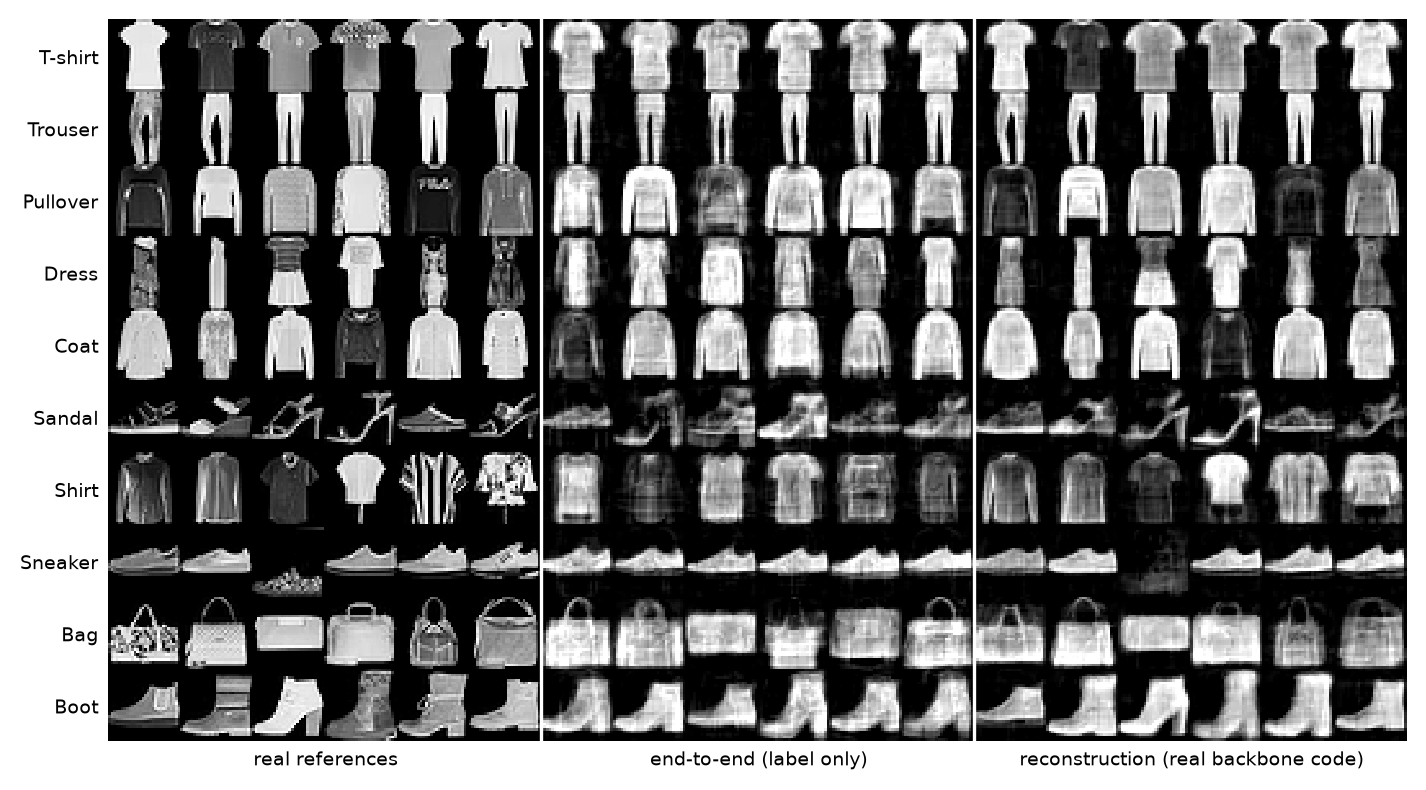
\includegraphics[width=\columnwidth]{figures/fig-samples.png}
\caption{\textbf{Emulated samples.} Real Fashion-MNIST references
(left), end-to-end draws from the label alone (center), and the
reconstruction control in which a real backbone code is supplied and
only the patch level and joint sweep run (right). Six per class, the
first six samples of one seed, with no selection.}
\label{fig:samples}
\end{figure}

\section{What was shown}

Every result is emulated lane computation on the open
\texttt{ktram-neural-core} runtime \cite{knowm2026emulator}: device
models with the read-noise physics above, every read and adapt issued
as a lane instruction, and decoding and scoring in host floating point.
The memristors and unit crossbars exist as fabricated, commercially
sold parts \cite{knowm2026datasheet}. The lane-scale system does not.

\subsection{Grayscale generation}

On grayscale Fashion-MNIST \cite{xiao2017fashion} the two-level system
was scored by a frozen pixel classifier for label agreement, plus
within-class diversity, tone spread, and contrast. End-to-end draws
from the label alone score 0.90 on the critic against 0.89 for real
images, with slightly higher diversity than real, lower tone spread,
and contrast about 14\% above real. The critic score is label
agreement and not a claim that the images equal real ones. Over 5120
drawn images every code is distinct, none is a copy of a training
image, and nearest-neighbor distances to the training set sit at or
beyond those of held-out real images. The generator is not memorizing.

\subsection{The comparator sweep}

Sweeping the comparator's noise setting with everything else fixed is
the paper's central experiment (Fig.~\ref{fig:sweep}). Every
binary-trained configuration with comparator noise below 20\% of the
read voltage, including the device-only point, fails the diversity
screen. Adding
comparator noise improves both stacks, with the grayscale critic best
at 20\% of the read voltage and binary FID best at 20 to 30\%. Raising
the read voltage fivefold at fixed comparator ratio, which cuts lane
thermal noise fivefold, leaves the metrics essentially unchanged. The
comparator ratio, not the device physics, is the sampling temperature.

This yields a concrete design requirement for a circuit that has not
yet been designed. The comparator's input-referred noise must be
adjustable from near zero to about 20 to 30\% of the read voltage, and
its static offset must be trimmed below about 10\% of the read voltage
at every bias setting: 1\,mV at a 10\,mV read. A raw dynamic latch has
the right noise range but carries 5 to 20\,mV of offset, and an
auto-zeroed or chopped comparator has the right offset but too little
noise. Neither class meets both requirements on its own, which is why
a per-lane trim plus a settable noise source is specified. A control
run also showed that replacing the idealized noiseless cold reads with
a physical noise floor flips some decisions but leaves every aggregate
metric unchanged.

\begin{figure}
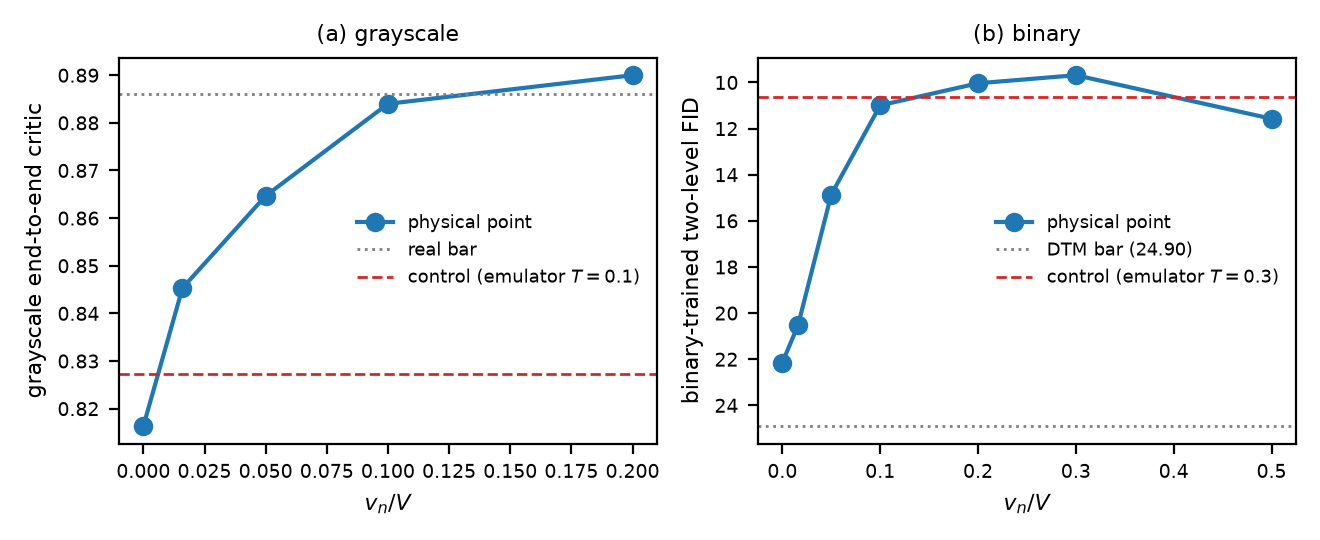
\includegraphics[width=\columnwidth]{figures/fig-comparator-sweep.png}
\caption{\textbf{The comparator's noise setting is the draw
temperature.} (a) Grayscale critic score against comparator noise
relative to read voltage, with the real-image score as a line. (b) The
same sweep on the binary-trained stack scored as FID, with the
published DTM value as a line. Lower FID is better.}
\label{fig:sweep}
\end{figure}

\subsection{Head-to-head with the DTM on binarized Fashion-MNIST}

The DTM paper reports quality as FID on binarized Fashion-MNIST but
does not state its sample count, feature extractor, or binarization
threshold, and its released library contains no FID code. That
library links to a replication repository \cite{dtmreplication} with
evaluation code and reference statistics, and we adopted that
protocol without modification. As a check, all 60\,000 real training
images binarized at the replication's threshold score FID 0.00004
against its shipped statistics, which fixes every element of the
scoring path at once. The DTM values in Table~\ref{tab:h2h} are
transcribed from the published paper and were not rerun.

\begin{table}
\caption{Binarized Fashion-MNIST under the replication protocol. DTM
rows are published values. Energies are modeled, not measured. Lower
FID is better.\label{tab:h2h}}
\begin{ruledtabular}
\footnotesize
\begin{tabular}{lcc}
system & FID & J/image (modeled) \\
\colrule
real fitting images (control) & 1.9 & --- \\
\colrule
CHILL ZEN two-level, grayscale-trained & 18.1 & $2.0\times10^{-9}$ \\
CHILL ZEN one-level, 128 books & 22.1 & $7.5\times10^{-10}$ \\
CHILL ZEN one-level, 64 books & 22.6 & $2.5\times10^{-10}$ \\
CHILL ZEN one-level, 32 books & 25.8 & $9.9\times10^{-11}$ \\
\colrule
CHILL ZEN two-level, binary-trained & \textbf{9.7} & $2.0\times10^{-9}$ \\
\colrule
DTM, 8 steps \cite{jelincic2025dtm} & 24.9 & $1.57\times10^{-8}$ \\
DTM, 2 steps \cite{jelincic2025dtm} & 32.6 & $3.92\times10^{-9}$ \\
\end{tabular}
\end{ruledtabular}
\end{table}

Two results stand out. The grayscale-trained system, with weights
unchanged and its renders simply thresholded, scores 18.1 against the
DTM's 24.9. Training the same architecture directly on binary images,
which removes an information asymmetry in the grayscale path, lowers
FID to 9.7 at the same modeled energy. The smaller one-level systems
trace an energy-quality frontier: 128 and 64 books clear the DTM bar at
a fraction of the energy, and 32 and 16 books do not. Drawing with the
class chosen at random rather than clamped raises FID by less than half
a point. A trivial independent-pixel sampler under the same protocol
scores 180, so the protocol does discriminate.

For context, the DTM paper's own baselines report 26.3 for a GAN, 17.9
for a VAE, and about 12 to 16 for a small diffusion model, none of
which we could verify. CHILL ZEN's 9.7 is in that company. One further
caution deserves emphasis: the binarization threshold alone moves FID
by more than the gap between any two systems. Real training images
binarized at the midpoint rather than at 0.1 score 29.8 against the
same reference, worse than the DTM. A number scored under an unstated
data convention is not comparable to anything.

\section{Energy and speed}

Both systems get their randomness from a circuit at every node, so
what separates them is how many random draws an image needs. CHILL
ZEN uses about 3600 hot lane reads. The eight-step DTM chain at its
stated 250 mixing iterations uses about $10^{7}$ conditional updates.
The two systems do different work per step, so the paper builds a
physical energy model from a stated geometry: one $4 \times 4$ unit
crossbar per address space on a 50\,nm pitch, addresses broadcast on
select lines across each bank, and one comparator per lane. Every
constant is a stated dimension or a textbook value, with no fitted
parameter. The model counts address delivery, divider reads, and
readout, applied to the deployed system's exact operation count of
10\,064 lane reads. It includes the decoder, counted as the 784 cold
lane reads it is designed to be.

\begin{table}
\caption{Modeled energy per image against the published eight-step DTM
chain at $1.57\times10^{-8}$\,J. These are scenario calculations from
the stated geometry, not measurements or uncertainty
bounds.\label{tab:energy}}
\begin{ruledtabular}
\begin{tabular}{lcc}
operating point & J/image & DTM ratio \\
\colrule
nominal: $4 \times 4$ array, 0.8\,V select & $2.0\times10^{-9}$ & $7.9\times$ \\
selector column, no sneak paths & $1.6\times10^{-9}$ & $9.9\times$ \\
low-swing select, 0.5\,V & $8.8\times10^{-10}$ & $17.7\times$ \\
7\,nm-class periphery, 0.5\,V & $4.2\times10^{-10}$ & $37\times$ \\
pessimistic corner & $8.1\times10^{-9}$ & $1.9\times$ \\
\end{tabular}
\end{ruledtabular}
\end{table}

At the nominal point the estimate is $2\times10^{-9}$\,J per image,
about one eighth of the DTM chain (Table~\ref{tab:energy}). Address
delivery at logic voltage is 91\% of that budget, which is the same
communication term the DTM paper reports as about half of its own.
Single-knob sensitivities move the ratio between about 4.6 and 7.9,
and the pessimistic corner still leaves the DTM at about twice CHILL
ZEN's energy. The advantage comes from doing less sampling work, not
from a cheaper random bit: the comparator's roughly 10\,fJ per read is
more expensive than the DTCA's measured 350\,aJ per random bit. Fewer
draws win by a wider margin than the per-draw cost loses.

On latency, the DTCA waits on its random-number generators, at about
$400\,\mu$s of sampling per image for the eight-step chain. CHILL ZEN
needs 131 sequential steps plus one parallel decode. If each step fits
the 62.5\,ns window used to budget readout energy, an image takes about
$8\,\mu$s, roughly fifty times faster. That window does not yet
establish a complete instruction cycle, so it is an illustration and
not a bound.

\begin{figure}
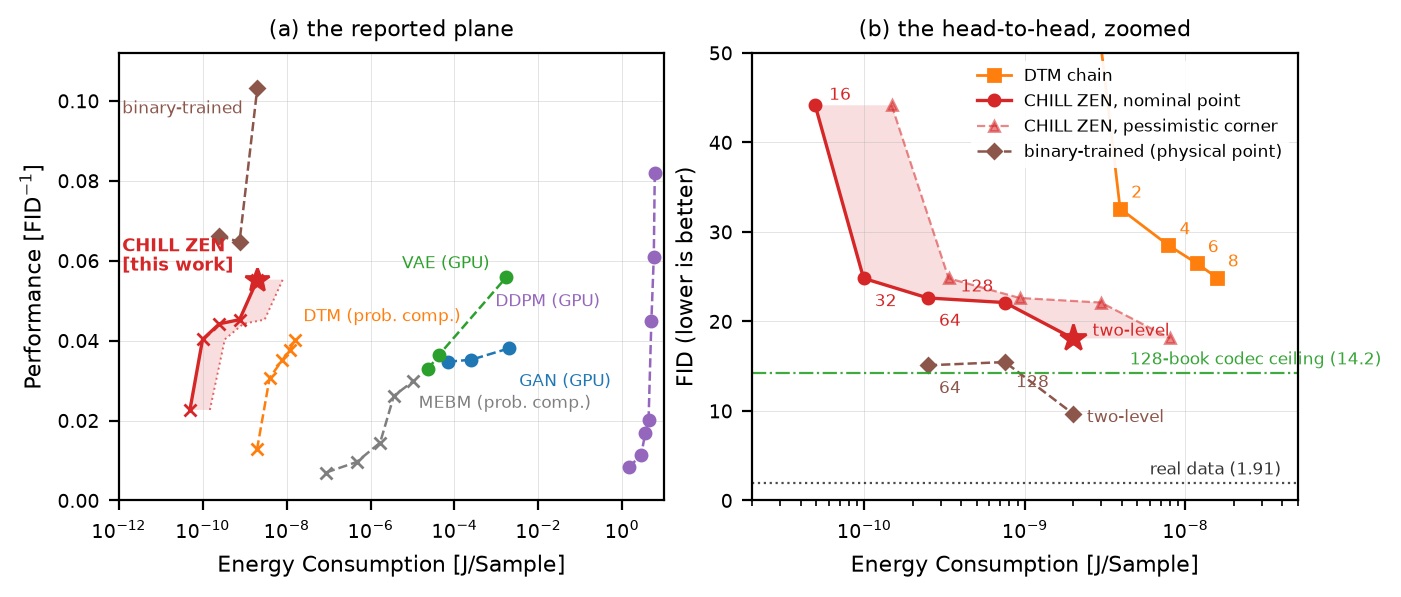
\includegraphics[width=\columnwidth]{figures/fig-energy.png}
\caption{\textbf{Quality against modeled energy.} (a) The axes of the
DTM paper's summary figure with its five published series re-plotted,
and the CHILL ZEN frontier added: one-level systems of 16 to 128 books
and the two-level system (star), with the shaded band extending each
point to the model's pessimistic corner. Binary-trained arms are
diamonds. (b) The same frontier against the DTM chain alone, drawn as
FID so the margin is readable. CHILL ZEN energies are model estimates.}
\label{fig:energy}
\end{figure}

\section{What is established, modeled, or open}

The claims in this document rest on three different kinds of
evidence, and a reader deciding what to make of them should keep the
three apart.

\emph{Established in emulation.} The architecture generates
recognizable, diverse, non-memorized images from a fixed sequence of
noisy reads with no equilibrium phase. Pooled device noise is
insufficient for sampling and the comparator must supply the
temperature. The comparator's noise ratio behaves as a temperature
knob with a clear optimum. Under a verified scoring path the emulated
system beats the published DTM FID, at 18.1 or 9.7 against 24.9. The
banks were taught by local lane instructions without gradients. The
emulator is bit-exact against the reference lane core, and every
number traces to a script in the released repository.

\emph{Modeled, not measured.} All energy figures come from a stated
geometry with textbook constants. They exclude weight programming, die
area, and leakage beyond a stated bound, as the DTM's own accounting
also excludes its programming. The nominal crossbar floats its
unselected lines and therefore has sneak paths, which the emulator
does not model; the selected symbol would contribute only 44\% of the
read conductance. The geometry the paper says it would build, a
$16 \times 1$ selector column, has no sneak path and models at
$1.6\times10^{-9}$\,J per image. The comparator is a specification and
not a circuit. Its bandwidth, noise, and energy have not been
demonstrated together in one design, and its kickback is unresolved.
The lane-side decoder has not been emulated at memristor precision.

\emph{Open.} The lane-scale system has not been fabricated. The
emulator's device noise constants are placeholders pending measurement.
The reported scores are validation numbers: the evaluation partition
informed epoch and noise-level selection, and each row is reported at
its best comparator setting on a declared grid. The training splits
differ from the DTM's in size and membership. There is no
gradient-trained baseline on the same code and connectivity, so the
paper does not claim that the local rule outperforms gradient
training. The remaining quality gap to real data, at FID 9.7 against a
reconstruction reference of 2.8, is unexplained.

\section{Bottom line}

CHILL ZEN reframes in-memory generative computing around a single
observation: once weights are pooled on a lane, the memory is too
quiet to sample itself, so the periphery must supply the temperature,
and a comparator whose noise is set per instruction does that job at
the point of readout. With that one knob, generation becomes a short,
fixed sequence of hot reads and cold sweeps rather than an equilibrium
chain, and the sampling count per image falls by more than three
orders of magnitude relative to the published DTM. In emulation this
delivers better FID than the DTM at about one eighth of its modeled
energy, and the frontier of smaller systems shows the trade-off is
tunable. What separates this from a product is a fabricated lane array
with selector columns, a comparator that meets the stated noise and
offset specification, and measured rather than modeled device
constants. Those are the next steps, and each is a circuit-engineering
task with a stated target rather than an open research question.

The full paper, code, saved evidence, and a map from every reported
number to the script that produces it are prepared for release at
\url{https://github.com/knowm/CHILL-ZEN}, with the lane emulator at
\url{https://github.com/knowm/ktram-neural-core}. The kT-bit, the
kT-RAM architecture, and its technology stack are the subject of
granted U.S. patents
\cite{nugent2015ktbitpatent,nugent2017ktrampatent,nugent2019stackpatent},
listed at \url{https://knowm.ai/ip/}. The author is part of Knowm
Inc., which has made and sold memristors and plans to sell products or
intellectual property based on the technologies described here.

\bibliography{refs}

\end{document}
